\documentclass[12pt,a4paper]{article}
\usepackage[utf8]{inputenc} %polskie znaki
\usepackage[T1]{fontenc}	%polskie znaki
\usepackage{amsmath}		%matematyczne znaczki :3
\usepackage{enumerate}		%Dodatkowe opcje do funkcji enumerate
\usepackage{geometry} 		%Ustawianie marginesow
\usepackage{graphicx}		%Grafika
\usepackage{wrapfig}		%Grafika obok textu
\usepackage{float}			%Allows H in fugire
\usepackage{xcolor}     	% for colour
\usepackage{lipsum}     	% for sample text
\usepackage{ntheorem}   	% for theorem-like environments
\usepackage{mdframed}   	% for framing
%\usepackage{amsthm}		%Dodaje przerwa u góry w twierdzeniach
%\pagestyle{empty} 			%usuwa nr strony

\theoremstyle{break}
\theoreminframepreskip{0.5cm}
\theoremheaderfont{\bfseries}
\newmdtheoremenv[%
linecolor=white,%
innertopmargin=\topskip,
shadowsize=0,%
innertopmargin=5,%
innerbottommargin=5,%
leftmargin=10,%
rightmargin=10,%
backgroundcolor=gray!20,%
innertopmargin=0pt,%
ntheorem]{zad}{Zadanie}


\newgeometry{tmargin=2cm, bmargin=2cm, lmargin=2cm, rmargin=2cm} 

\begin{document}
	
	\begin{center}
		\LARGE Funkcja wykładnicza i logarytmiczna - karta pracy
	\end{center}
	
	\begin{tabular}{p{13cm} r}
		Imię i nazwisko: ............................................................................
		&[....../22pkt]\\ 
		\vspace{0.5cm}
	\end{tabular}

	\begin{zad}[0-3]
		\textbf{Zapisz poniższe wyrażenia w postaci} $a^x$ \textbf{.}
	\end{zad} 
	
	\begin{enumerate}[a)]\Large
		\item $\frac{3^5:(3^2)^3}{(3^{-2})^5}=$
		\item $\frac{2^9\cdot4^5}{8^4}=$
		\item $\frac{6^7\cdot12^{-4}}{8}=$
	\end{enumerate}
	
	%%%%%%%%%%%%%%%%%%%%%%%%%%%%%
	
	\begin{zad}[0-1]
		\textbf{Dokończ zdanie. Wybierz właściwą odpowiedź spośród podanych.}
	\end{zad} 
	
	Połowa liczby \Large$\frac{4^{150}\;\cdot\;4^{50}}{4^{100}}\:$\normalsize wynosi:
	
	\vspace{0.5cm}
	\begin{tabular}{p{3.5cm} p{3.5cm} p{3.5cm} p{3.5cm}}
		\textbf{A. }$2^{100}$&
		\textbf{B. }$2^{50}$&
		\textbf{C. }$2^{199}$&
		\textbf{D. }$4^{50}$\\
	\end{tabular}

	%%%%%%%%%%%%%%%%%%%%%%%%%%%%%
	
	\begin{zad}[0-3]
		\textbf{Wykaż, że liczba:}
		$$k=5^{120}+6\cdot5^{119}+7\cdot5^{118}$$
		\textbf{jest podzielna przez 16.}
	\end{zad} 


	\begin{tabular}{|p{0.1cm}|p{0.1cm}|p{0.1cm}|p{0.1cm}|p{0.1cm}|p{0.1cm}|p{0.1cm}|p{0.1cm}|p{0.1cm}|p{0.1cm}|p{0.1cm}|p{0.1cm}|p{0.1cm}|p{0.1cm}|p{0.1cm}|p{0.1cm}|p{0.1cm}|p{0.1cm}|p{0.1cm}|p{0.1cm}|p{0.1cm}|p{0.1cm}|p{0.1cm}|p{0.1cm}|p{0.1cm}|p{0.1cm}|p{0.1cm}|p{0.1cm}|p{0.1cm}|p{0.1cm}|p{0.1cm}|p{0.1cm}}
		\hline&&&&&&&&&&&&&&&&&&&&&&&&&&&&&&\\
		\hline&&&&&&&&&&&&&&&&&&&&&&&&&&&&&&\\
		\hline&&&&&&&&&&&&&&&&&&&&&&&&&&&&&&\\
		\hline&&&&&&&&&&&&&&&&&&&&&&&&&&&&&&\\
		\hline&&&&&&&&&&&&&&&&&&&&&&&&&&&&&&\\
		\hline&&&&&&&&&&&&&&&&&&&&&&&&&&&&&&\\
		\hline&&&&&&&&&&&&&&&&&&&&&&&&&&&&&&\\
		\hline&&&&&&&&&&&&&&&&&&&&&&&&&&&&&&\\
		\hline&&&&&&&&&&&&&&&&&&&&&&&&&&&&&&\\
		\hline&&&&&&&&&&&&&&&&&&&&&&&&&&&&&&\\
		\hline&&&&&&&&&&&&&&&&&&&&&&&&&&&&&&\\
		\hline&&&&&&&&&&&&&&&&&&&&&&&&&&&&&&\\
		\hline&&&&&&&&&&&&&&&&&&&&&&&&&&&&&&\\
		\hline&&&&&&&&&&&&&&&&&&&&&&&&&&&&&&\\
		\hline&&&&&&&&&&&&&&&&&&&&&&&&&&&&&&\\
		\hline&&&&&&&&&&&&&&&&&&&&&&&&&&&&&&\\
		\hline&&&&&&&&&&&&&&&&&&&&&&&&&&&&&&\\
		\hline
	\end{tabular}
	

	
	\newpage
	%%%%%%%%%%%%%%%%%%%%%%%%%%%%%
	
			\begin{mdframed}[%
		linecolor=white,%
		innertopmargin=\topskip,
		shadowsize=0,%
		innertopmargin=5,%
		innerbottommargin=5,%
		leftmargin=10,%
		rightmargin=10,%
		backgroundcolor=gray!20,%
		innertopmargin=0pt,]
		\vspace{0.2cm}
		\textbf{\textit{Informacja do zadań 4-5.}}
		
		
	\end{mdframed}

		Poniżej przedstawiono wykres funkcji wykładniczej, której wzór wyraża się w postaci $$f(x)=a^x.$$
	
	\begin{figure}[h]
		\centering
		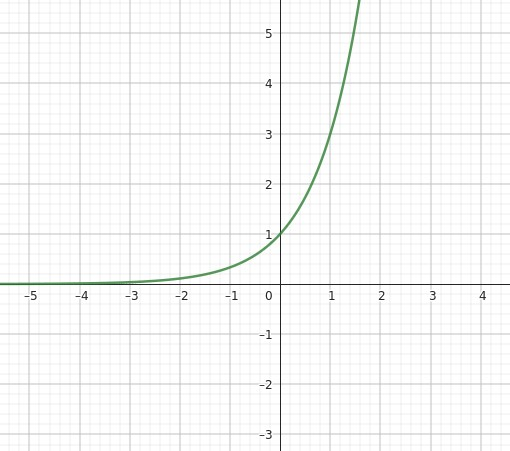
\includegraphics[scale=0.7]{r1.jpeg}
	\end{figure}

	%%%%%%%%%%%%%%%%%%%%%%%%%%%%%
	
	\begin{zad}[0-1]
		\textbf{Dokończ zdanie. Wybierz właściwą odpowiedź spośród podanych.}
	\end{zad} 
	
	Wartość wyrażenia $f(1)-f(0)$ jest równa:
	
	\vspace{0.5cm}
	\begin{tabular}{p{3.5cm} p{3.5cm} p{3.5cm} p{3.5cm}}
		\textbf{A. }$1$&
		\textbf{B. }$2$&
		\textbf{C. }$-2$&
		\textbf{D. }$3$\\
	\end{tabular}

	%%%%%%%%%%%%%%%%%%%%%%%%%%%%%

	\begin{zad}[0-3]
		\textbf{Wyznacz współczynnik "a" powyższej funkcji wykładniczej.}
	\end{zad} 
	
		\begin{tabular}{|p{0.1cm}|p{0.1cm}|p{0.1cm}|p{0.1cm}|p{0.1cm}|p{0.1cm}|p{0.1cm}|p{0.1cm}|p{0.1cm}|p{0.1cm}|p{0.1cm}|p{0.1cm}|p{0.1cm}|p{0.1cm}|p{0.1cm}|p{0.1cm}|p{0.1cm}|p{0.1cm}|p{0.1cm}|p{0.1cm}|p{0.1cm}|p{0.1cm}|p{0.1cm}|p{0.1cm}|p{0.1cm}|p{0.1cm}|p{0.1cm}|p{0.1cm}|p{0.1cm}|p{0.1cm}|p{0.1cm}|p{0.1cm}}
		\hline&&&&&&&&&&&&&&&&&&&&&&&&&&&&&&\\
		\hline&&&&&&&&&&&&&&&&&&&&&&&&&&&&&&\\
		\hline&&&&&&&&&&&&&&&&&&&&&&&&&&&&&&\\
		\hline&&&&&&&&&&&&&&&&&&&&&&&&&&&&&&\\
		\hline&&&&&&&&&&&&&&&&&&&&&&&&&&&&&&\\
		\hline&&&&&&&&&&&&&&&&&&&&&&&&&&&&&&\\
		\hline&&&&&&&&&&&&&&&&&&&&&&&&&&&&&&\\
		\hline&&&&&&&&&&&&&&&&&&&&&&&&&&&&&&\\
		\hline&&&&&&&&&&&&&&&&&&&&&&&&&&&&&&\\
		\hline&&&&&&&&&&&&&&&&&&&&&&&&&&&&&&\\
		\hline&&&&&&&&&&&&&&&&&&&&&&&&&&&&&&\\
		\hline&&&&&&&&&&&&&&&&&&&&&&&&&&&&&&\\
		\hline&&&&&&&&&&&&&&&&&&&&&&&&&&&&&&\\
		\hline&&&&&&&&&&&&&&&&&&&&&&&&&&&&&&\\
		\hline&&&&&&&&&&&&&&&&&&&&&&&&&&&&&&\\
		\hline
	\end{tabular}
	
	%%%%%%%%%%%%%%%%%%%%%%%%%%%%%
	
	\begin{zad}[0-1]
		\textbf{Dokończ zdanie. Wybierz właściwą odpowiedź spośród podanych.}
	\end{zad} 
	
	Wyrażenie $\sqrt{5\sqrt[3]{5}}$ można zapisać w postaci:
	
	\vspace{0.5cm}
	\begin{tabular}{p{3.5cm} p{3.5cm} p{3.5cm} p{3.5cm}}
		\textbf{A. }$5$&
		\textbf{B. }$5^{-6}$&
		\textbf{C. }$5^\frac{1}{6}$&
		\textbf{D. }$5^\frac{1}{2}$\\
	\end{tabular}	

	%%%%%%%%%%%%%%%%%%%%%%%%%%%%%
	
	\begin{zad}[0-3]
		\textbf{Oblicz:}
	\end{zad} 
	
	\begin{enumerate}[a)]
		\item $\sqrt{8}+\sqrt{18}+\sqrt{32}=$
		\item $4\sqrt{7}-3\sqrt{63}+2\sqrt{28}=$
		\item $3\sqrt{3}\cdot2\sqrt{6}+\frac{6\sqrt{4}}{\sqrt{2}}-7\sqrt{18}=$
	\end{enumerate}

	%%%%%%%%%%%%%%%%%%%%%%%%%%%%%
	
	\begin{zad}[0-1]
		\textbf{Dokończ zdanie. Wybierz właściwą odpowiedź spośród podanych.}
	\end{zad} 
	
	Wartość wyrażenia $\log_2(8\sqrt{2})$ wynosi:
	
	\vspace{0.5cm}
	\begin{tabular}{p{3.5cm} p{3.5cm} p{3.5cm} p{3.5cm}}
		\textbf{A. }$2$&
		\textbf{B. }$3\frac{1}{2}$&
		\textbf{C. }$4\frac{1}{2}$&
		\textbf{D. }$7$\\
	\end{tabular}
	
	%%%%%%%%%%%%%%%%%%%%%%%%%%%%%
	
	\begin{zad}[0-2]
		\textbf{Oblicz:}
	\end{zad} 
	
	\begin{enumerate}[a)]
		\item $5\log0,01=$
		\item $\log_3(\log_28)=$
	\end{enumerate}
	
	%%%%%%%%%%%%%%%%%%%%%%%%%%%%%
	
	\begin{zad}[0-1]
		\textbf{Dokończ zdanie. Wybierz właściwą odpowiedź spośród podanych.}
	\end{zad} 
	
	Wyrażenie $\log_{12} 6 + \log_{12} 24$ jest równe:
	
	\vspace{0.5cm}
	\begin{tabular}{p{3.5cm} p{3.5cm} p{3.5cm} p{3.5cm}}
		\textbf{A. }$2$&
		\textbf{B. }$2\frac{1}{2}$&
		\textbf{C. }$\log_{12}30$&
		\textbf{D. }$3$\\
	\end{tabular}



	%%%%%%%%%%%%%%%%%%%%%%%%%%%%%
	
	\begin{zad}[0-3]
		\textbf{Oblicz:}
	\end{zad} 
	
	\begin{enumerate}[a)]
		\item $3\log5+\log8=$
		\item $\log_6216+\log_464=$
		\item $\log_327-3\log_3\frac{1}{3}+\log_31=$
	\end{enumerate}
	
\end{document}